\documentclass[a4paper, 14pt]{extarticle}

\usepackage[T2A]{fontenc}
\usepackage{natbib}
\usepackage{graphicx}
\usepackage[english, russian]{babel}
\usepackage{fontspec}
\usepackage{amsmath}
\usepackage{amsfonts}
\usepackage{amssymb}
\usepackage{amsthm}
\usepackage{mathtools}
\usepackage{mathrsfs}
\usepackage{icomma}
\usepackage{fullpage}
\usepackage{ulem}
\usepackage{setspace}
\usepackage{listings}
\usepackage{indentfirst}
\usepackage[left=2cm,right=1.5cm,top=2cm,bottom=2cm]{geometry}
\usepackage{xcolor}
\usepackage{float}
\usepackage{csquotes}
\usepackage{hyperref}
\usepackage{graphics}



\definecolor{urlcolor}{HTML}{0000FF} % цвет гиперссылок
\definecolor{linkcolor}{HTML}{000000} % цвет гиперссылок
\hypersetup{pdfstartview=FitH, linkcolor=linkcolor, urlcolor=urlcolor, colorlinks=true}


\setmainfont{Times New Roman}
\setlength{\parindent}{5ex}
\setlength{\parskip}{1em}
\renewcommand{\baselinestretch}{1}

\graphicspath{{images/}}


\definecolor{buzzlightyear}{HTML}{8757A5}
\definecolor{grass}{HTML}{738D06}
\definecolor{literal}{HTML}{F18A2B}
\definecolor{commentcolor}{HTML}{8E908B}

\lstdefinestyle{habrstyle}{
    backgroundcolor=\color{white},
    commentstyle=\color{commentcolor},
    keywordstyle=\bfseries\color{buzzlightyear},
    numberstyle=\tiny\color{commentcolor},
    stringstyle=\color{grass},
    basicstyle=\ttfamily\footnotesize,
    breakatwhitespace=false,
    breaklines=true,
    captionpos=b,
    keepspaces=true,
    numbers=left,
    numbersep=5pt,
    showspaces=false,
    showstringspaces=false,
    showtabs=false,
    tabsize=4
}

\lstset{style=habrstyle}

\begin{document}
    % НАЧАЛО ТИТУЛЬНОГО ЛИСТА
    \begin{center}
        \begin{center}
            \hfill \break
            \normalsize{Санкт-Петербургский государственный политехнический}\\
            \normalsize{университет Петра Великого}\\
            \hfill \break
            \normalsize{\textbf{Высшая школа интеллектуальных систем и}}\\
            \normalsize{\textbf{суперкомпьютерных технологий}}\\
            \hfill \break
            \hfill \break
            \hfill \break
            \normalsize{Лабораторная работа}\\
            \hfill \break
            \normalsize{\LARGE Гармоники}\\
        \end{center}
        \hfill \break
        \hfill \break
        \hfill \break
        \hfill \break
        \hfill \break
        \hfill \break
        \hfill \break
        \hfill \break
        \hfill \break
        \hfill \break
        \begin{tabbing}
            Выполнил студент гр. 3530901/80201 \`И.С. Иванов\\
            \\
            Преподаватель: \`Н.В. Богач\\
        \end{tabbing}
        \hfill \break
        \hfill \break
        \hfill \break
        \hfill \break
        \begin{center}
            Санкт-Петербург\\
            2021
        \end{center}
        \thispagestyle{empty}
    \end{center}
    % КОНЕЦ ТИТУЛЬНОГО ЛИСТА

    % ОГЛАВЛЕНИЕ
    \newpage
    \tableofcontents

    % СПИСОК ИЛЛЮСТРАЦИЙ
    \newpage
    \listoffigures

    % СПИСОК ЛИСТИНГОВ
    \newpage
    \lstlistoflistings

    \newpage


    \section{Упражнение №1: Изучить примеры из chap02}
    \label{sec:1_study_examples}

    Для выполнения первого пункта необходимо изучить и выполнить примеры из файла chap02.ipynb.
    Запустим все примеры из этого файла.

    \begin{figure}[h]
        \centering
        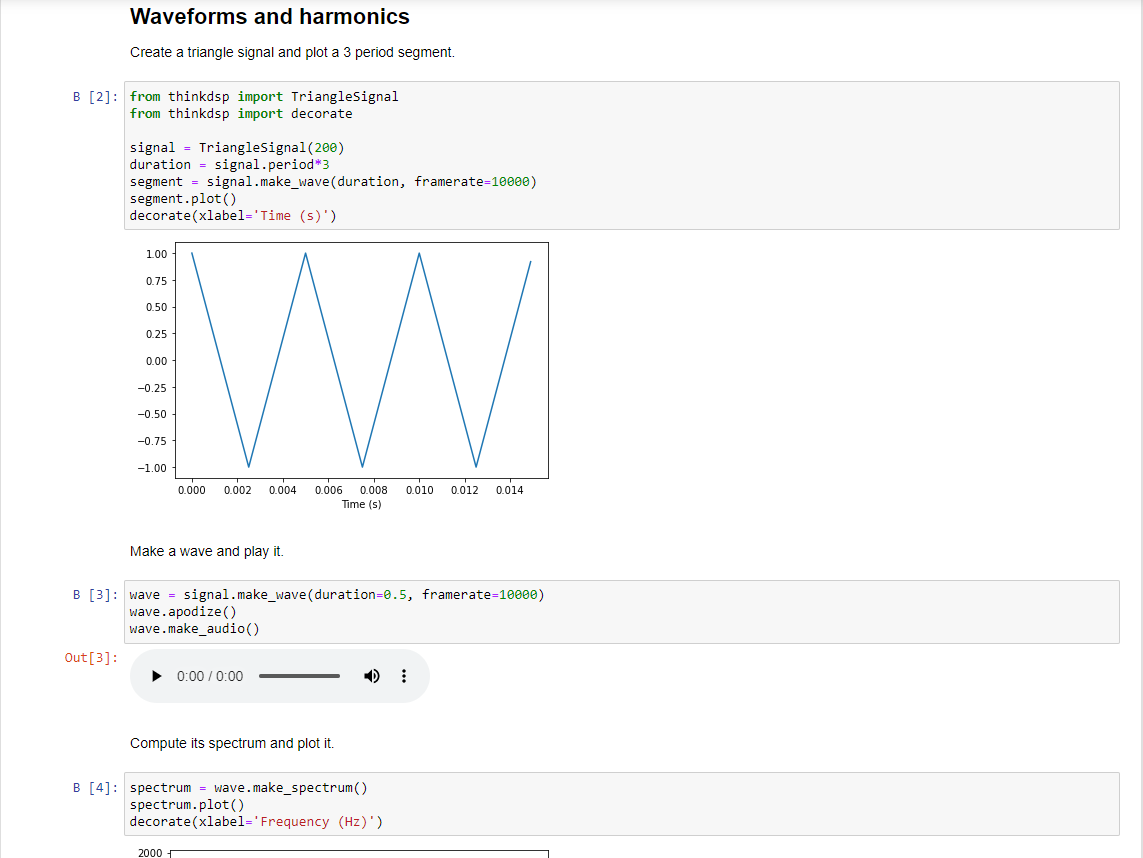
\includegraphics[width=\textwidth]{chap02_1}
        \caption{Изучение и проверка примеров из файла (1)}
        \label{fig:check_it_works_1}
    \end{figure}

    \begin{figure}[h]
        \centering
        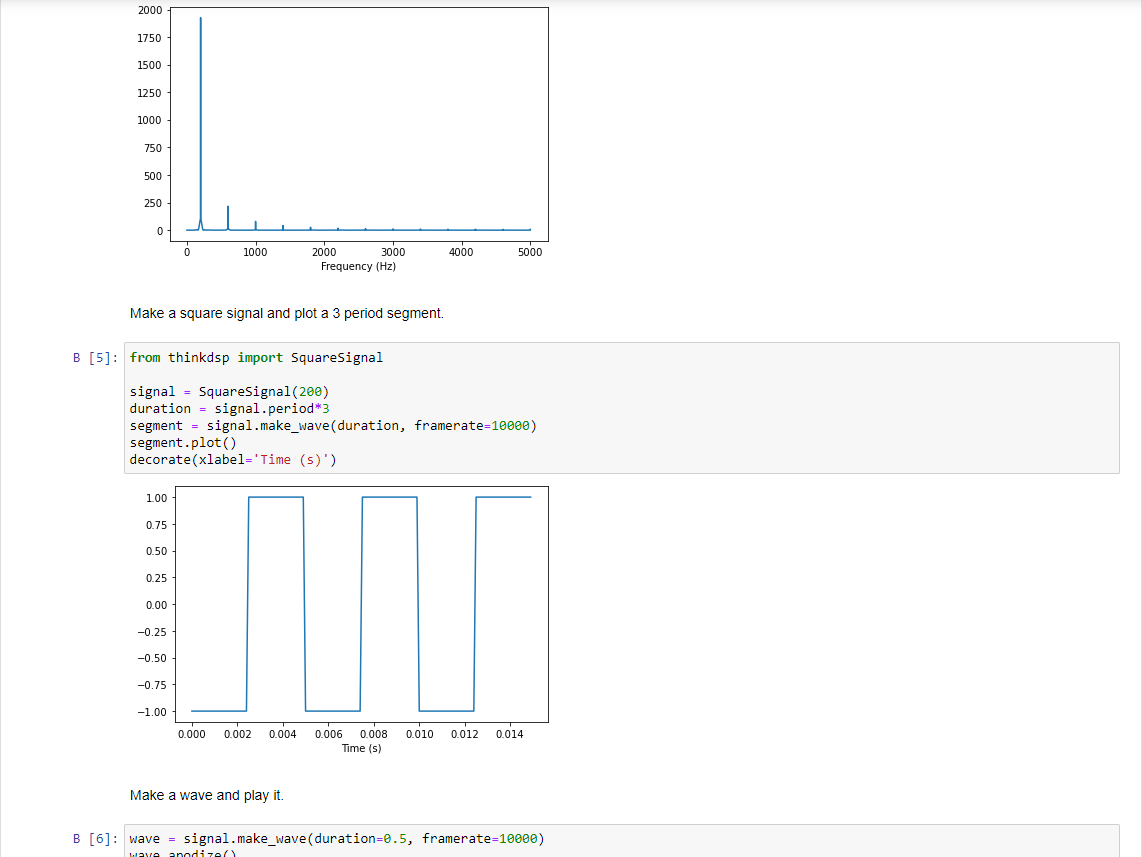
\includegraphics[width=\textwidth]{chap02_2}
        \caption{Изучение и проверка примеров из файла (2)}
        \label{fig:check_it_works_2}
    \end{figure}

    \newpage


    \section{Упражнение №2: SawtoothSignal}
    \label{sec:2_sawtooth_signal}

    Во втором упражнении необходимо написать класс SawtoothSignal, расширяющий signal и предоставляющий evaluate для оценки пилообразного сигнала

    Подключение зависимостей и написание класса SawtoothSignal:

    \begin{lstlisting}[language=Python, caption= Класс SawtoothSignal, label={lst:sawtooth_code}]
        from thinkdsp import Sinusoid
        from thinkdsp import normalize, unbias
        import numpy as np

        class SawtoothSignal(Sinusoid):

            def evaluate(self, ts):
                cycles = self.freq * ts + self.offset / np.pi / 2
                frac, _ = np.modf(cycles)
                ys = normalize(unbias(frac), self.amp)
                return ys

    \end{lstlisting}

    Проверим работу класса.
    Выведем график сигнала и послушаем получившийся wav:

    \begin{lstlisting}[language=Python, caption= Вывод графика и создание wav, label={lst:create_wav_plot}]
        saw_wav = SawtoothSignal().make_wave(duration=0.5, framerate=40000)
        saw_wav.segment(start=0, duration=0.01).plot()
        saw_wav.make_audio()

    \end{lstlisting}

    \begin{figure}[H]
        \centering
        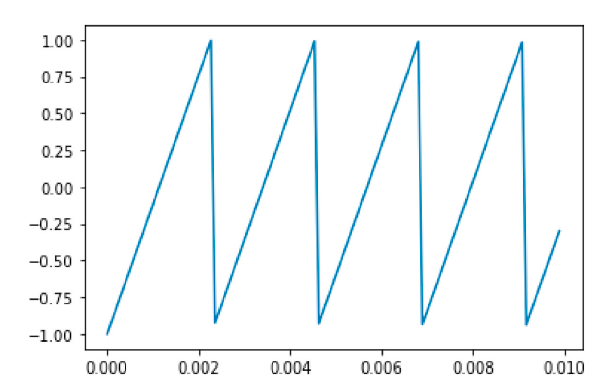
\includegraphics[width=\textwidth]{sawtooth_plot}
        \caption{График sawtooth}
        \label{fig:sawtooth_plot}
    \end{figure}

    Выведем спектр:

    \begin{lstlisting}[language=Python, caption= Вывод спектра sawtooth, label={lst:sawtooth_spectr}]
        saw_wav.make_spectrum().plot()
    \end{lstlisting}

    \begin{figure}[H]
        \centering
        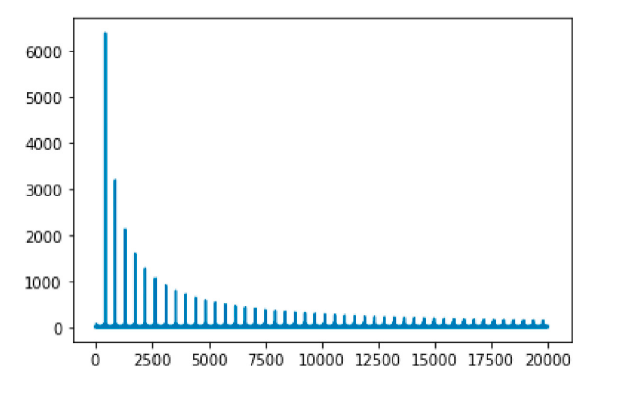
\includegraphics[width=\textwidth]{sawtooth_spectr}
        \caption{Спектр sawtooth}
        \label{fig:sawtooth_spectr}
    \end{figure}

    Сравним наш пилообразный сигнал с прямоугольным

    \begin{lstlisting}[language=Python, caption= Изображение спектра, label={lst:square_sawtooth_spectr_plot}]
        from thinkdsp import SquareSignal

        saw_wav.make_spectrum().plot(color='gray')
        square_wav = SquareSignal(amp=0.5).make_wave(duration=0.5, framerate=40000)
        square_wav.make_spectrum().plot()
    \end{lstlisting}

    \begin{figure}[H]
        \centering
        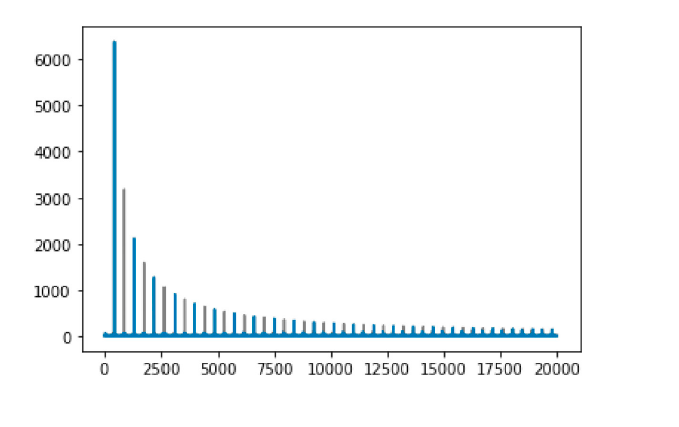
\includegraphics[width=\textwidth]{square_sawtooth_spectr}
        \caption{Прямоугольный и пилообразный спектр}
        \label{fig:square_sawtooth_spectr}
    \end{figure}

    Прослушаем прямоугольный сигнал:

    \begin{lstlisting}[language=Python, caption= Создание звука прямоугольного сигнала, label={lst:square_make_audio}]
        square_wav.make_audio()
    \end{lstlisting}

    Сравним наш пилообразный сигнал с треугольным:

    \begin{lstlisting}[language=Python, caption= Фильтрация спектра, label={lst:triangle_sawtooth_spectr_plot}]
        from thinkdsp import TriangleSignal

        saw_wav.make_spectrum().plot(color='gray')
        triangle_wav = TriangleSignal(amp=0.79).make_wave(duration=0.5, framerate=40000)
        triangle_wav.make_spectrum().plot()
    \end{lstlisting}

    \begin{figure}[H]
        \centering
        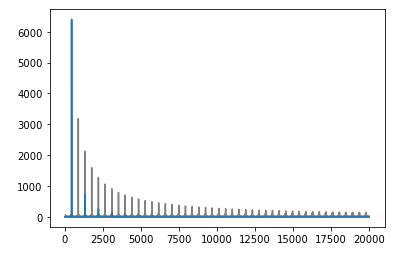
\includegraphics[width=\textwidth]{triangle_sawtooth_spectr}
        \caption{Отфильтрованный спектр}
        \label{fig:triangle_sawtooth_spectr}
    \end{figure}

    Прослушаем треугольный сигнал:

    \begin{lstlisting}[language=Python, caption= Перевод в аудио, label={lst:triangle_make_audio}]
        triangle_wav.make_audio()
    \end{lstlisting}

    По результатам выполнения данного упражнения можно сделать вывод, что по сравнению с прямоугольным сигналом, пилообразный уменьшается аналогично, но включает четные и нечетные гармоники.
    Гармоники треугольного сигнала уменьшаются пропорционально \(1/f^2\), а пилообразный уменьшается \(1/f\).

    \newpage


    \section{Упражнение №3: Квадратный сигнал}
    \label{sec:3_square_signal}

    В третьем упражнении нам необходимо создать квадратный сигнал частотой 1100 Гц и вычислить wave с выборками 10000 кадров в секунду.
    Построив спектр, убедимся, что большинство гармоник "завернуты" из-за биения.

    Создадим прямоугольный сигнал и выведем его спектр:

    \begin{lstlisting}[language=Python, caption= Создание сигнала и вывод его спектра, label={lst:gen_signal_plot}]
        square_wav1 = SquareSignal(1500).make_wave(duration=0.5, framerate=10000)
        square_wav1.make_spectrum().plot()
    \end{lstlisting}

    \begin{figure}[H]
        \centering
        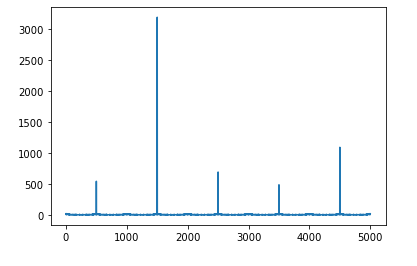
\includegraphics[width=\textwidth]{square_signal_spectr}
        \caption{Спектр прямоугольного сигнала}
        \label{fig:square_signal_spectr}
    \end{figure}

    После этого было получено аудио из данного сигнала:

    \begin{lstlisting}[language=Python, caption= Получение аудио, label={lst:make_audio_from_signal}]
        square_wav1.make_audio()
    \end{lstlisting}

    Для сравнения создадим синусоидальный сигнал частотой 500 Гц и выведем его спектр:

    \begin{lstlisting}[language=Python, caption= Создание синусоидального сигнала и получение его спектра, label={lst:make_sin_signal_spectr}]
        from thinkdsp import SinSignal

        sin_wav = SinSignal(500).make_wave(duration=0.5, framerate=10000)
        sin_wav.make_spectrum()
    \end{lstlisting}

    \begin{figure}[H]
        \centering
        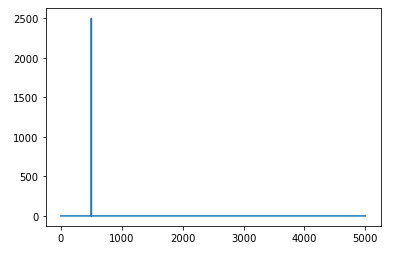
\includegraphics[width=\textwidth]{sin_spectr}
        \caption{Полученный спектр синусоидального сигнала}
        \label{fig:sin_signal_spectr}
    \end{figure}

    Получим аудио из данного сигнала:

    \begin{lstlisting}[language=Python, caption= Получение аудио, label={lst:sin_make_audio}]
        sin_wav.make_audio()
    \end{lstlisting}

    По результатам выполнения данного упражнения, сравнивая два сигнала, можно сделать вывод, что они похожи.
    Прослушивая первый сигнал и сравнивая со вторым, слышно что основной тон в первом сигнале, который мы слышим это "alias" частоты 500 Гц.

    \newpage


    \section{Упражнение №4: Нулевая частота}
    \label{sec:4_zero_freq}

    В четвертом упражнении необходимо взять объект \texttt{spectrum} и распечатать несколько первых значений \texttt{spectrum.hs}.
    Необходимо также убедиться, что они начинаются с нуля, т.е. \texttt{spectrum.hs[0]} - амплитуда компонента с частотой 0.

    \begin{enumerate}
        \item Создать треугольный сигнал с частотой 440Гц и \texttt{wave} длительностью 0.01с после чего вывести график сигнала.
        \item Создать объект \texttt{spectrum} и вывести \texttt{spectrum.hs[0]}.
        Определить какая амплитуда и фаза у компонента.
        \item Установить \texttt{spectrum.hs[0]} = 100 и определить как данная операция влияет на сигнал.
    \end{enumerate}

    Создадим треугольный сигнал и выведем его график:

    \begin{lstlisting}[language=Python, caption= Создание и вывод на экран треугольного сигнала, label={lst:make_triangle_signal_plot}]
        triangle = TriangleSignal().make_wave(duration=0.01)
        triangle.plot()
    \end{lstlisting}

    \begin{figure}[H]
        \centering
        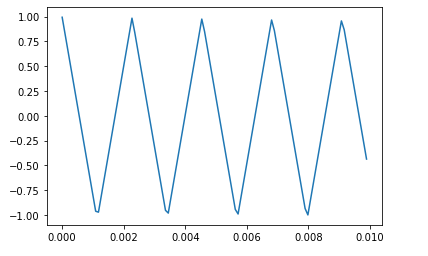
\includegraphics[width=\textwidth]{triangle_signal_plot}
        \caption{График треугольного сигнала}
        \label{fig:triangle_signal_plot}
    \end{figure}

    Создадим спектр сигнала и выведем spectrum.hs[0]

    \begin{lstlisting}[language=Python, caption= Создание спектра и вывод spectrum.hs, label={lst:create_spectrum_triangle_signal}]
        spectrum = triangle.make_spectrum()
        spectrum.hs[0]
    \end{lstlisting}

    Получившийся элемент спектра \texttt{(1.0436096431476471e-14+0j)} комплексное число, близкое к нулю.

    Установим \texttt{spectrum.hs[0]} = 100 и выведем сигнал на экран:

    \begin{lstlisting}[language=Python, caption= Изменение spectrum.hs и вывод сигналов на экран, label={lst:change_spectrum}]
        spectrum.hs[0] = 100
        triangle.plot(color='gray')
        spectrum.make_wave().plot()
    \end{lstlisting}

    \begin{figure}[H]
        \centering
        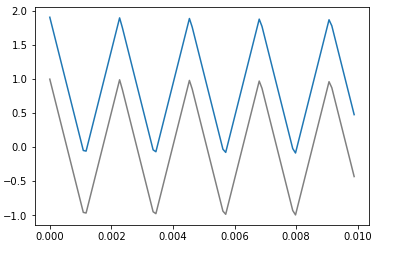
\includegraphics[width=\textwidth]{triangle_signal_spectr_change}
        \caption{График сигнала после изменения}
        \label{fig:triangle_signal_spectr_change}
    \end{figure}

    По результатам выполнения данного упражнения можно сделать вывод, что два сигнала не отличаются друг от друга, кроме уровня громкости.

    \newpage


    \section{Упражнение №5: Фильтрация спектра}
    \label{sec:5_spectrum_filter}

    В пятом упражнении необходимо написать функцию, принимающую \texttt{spectrum} как параметр и изменяющую его делением каждого элемента \texttt{hs} на соответствующую частоту из \texttt{fs}.
    Необходимо также проверить данную функцию на прямоугольном, треугольном или пилообразном сигнале.

    \begin{enumerate}
        \item Вычислить спектр и вывести его.
        \item Изменить спектр, используя функцию, и вывести его.
        \item Использовать \texttt{spectrum.make\_wave}, чтобы сделать \texttt{wave} из измененного спектра и прослушать его.
    \end{enumerate}

    Создадим функцию filter\_spectrum:

    \begin{lstlisting}[language=Python, caption= Функция filter\_spectrum, label={lst:filter_spectrum}]
        def filter_spectrum(s):
            s.hs[1:] /= s.fs[1:]
            s.hs[0] = 0
    \end{lstlisting}

    Создадим прямоугольный сигнал и переведем его в аудио:

    \begin{lstlisting}[language=Python, caption= Создание прямоугольного сигнала и создание аудио, label={lst:make_signal_audio}]
        square_wav2 = SquareSignal(freq=440).make_wave(duration=0.5)
        square_wav2.make_audio()
    \end{lstlisting}

    Выведем на экран исходный спектр.
    Изменим спектр с помощью нашей функции.
    Выведем измененный спектр.

    \begin{lstlisting}[language=Python, caption= Изменение и вывод спектров на экран, label={lst:change_spectr_with_func}]
        spectrum_square = square_wav2.make_spectrum()
        spectrum_square.plot(high=10000, color='gray')
        filter_spectrum(spectrum_square)
        spectrum_square.scale(440)
        spectrum_square.plot(high=10000)
    \end{lstlisting}

    \begin{figure}[H]
        \centering
        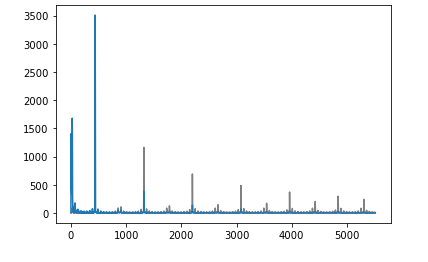
\includegraphics[width=\textwidth]{square_filtered_spectrum}
        \caption{Исходный и измененный спектр}
        \label{fig:square_filtered_spectrum}
    \end{figure}

    Переведем отфильтрованный спектр в аудио и прослушаем.

    По результатам выполнения данного упражнения можно сделать вывод, что полученный сигнал тише исходного и высокие частоты были отфильтрованы.


    \section{Упражнение №6: Создание сигнала}
    \label{sec:6_find_signal}

    В шестом упражнении необходимо определить, можно ли создать сигнал, состоящий из четных и нечетных гармоник, спадающих пропорционально \(1/f^2\).

    Создадим пилообразный сигнал и прослушаем его:

    \begin{lstlisting}[language=Python, caption= Создание пилообразного сигнала, label={lst:make_sawtooth_signal_audio}]
        freq = 500
        signal = SawtoothSignal(freq=freq)
        sawtooth_wave = signal.make_wave(duration=0.5, framerate=20000)
        sawtooth_wave.make_audio()
    \end{lstlisting}

    Выведем его спектр:

    \begin{lstlisting}[language=Python, caption= Спектр пилообразного сигнала, label={lst:sawtooth_spectrum_plot}]
        sawtooth_spectrum = sawtooth_wave.make_spectrum()
        sawtooth_spectrum.plot()
    \end{lstlisting}

    Необходимо отфильтровать спектр с помощью функции написанной раннее.
    После фильтрации выведем спектр на экран

    \begin{lstlisting}[language=Python, caption= Фильтрация и вывод спектра, label={lst:filter_spectrum_plot}]
        sawtooth_spectrum.plot(color='gray')
        filter_spectrum(sawtooth_spectrum)
        sawtooth_spectrum.scale(freq)
        sawtooth_spectrum.plot()
    \end{lstlisting}

    \begin{figure}[H]
        \centering
        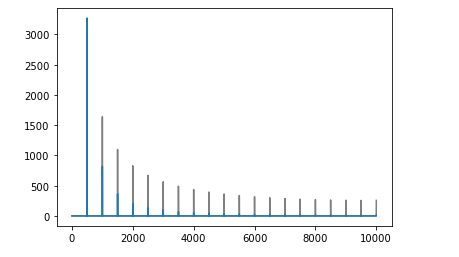
\includegraphics[width=\textwidth]{sawtooth_filtered_spectrum}
        \caption{Исходный и отфильтрованный спектр}
        \label{fig:sawtooth_filtered_spectrum}
    \end{figure}

    Далее переведем отфильтрованный спектр в аудио и прослушаем.

    После этого выделим сегмент из полученного сигнала отфильтрованного спектра длительностью 0.01 с.
    Выведем сигнал сегмента на экран.

    \begin{lstlisting}[language=Python, caption= Фильтрация и вывод спектра, label={lst:sawtooth_filtered_segment_plot}]
        temp_wave.segment(duration=0.01).plot()
    \end{lstlisting}

    \begin{figure}[H]
        \centering
        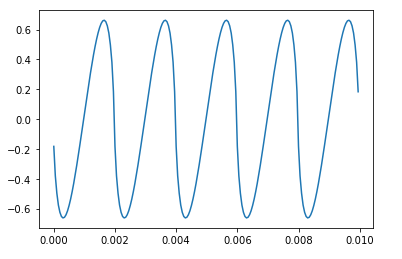
\includegraphics[width=\textwidth]{sawtooth_filtered_segment}
        \caption{Сигнал сегмента}
        \label{fig:sawtooth_filtered_segment}
    \end{figure}

    Данный сигнал не особо похож на какую либо математическую функцию.
    Поэтому выполним другой подход.
    Сложим серию косинусоидальных сигналов с правильными частотами и амплитудами.
    Отобразим спектр полученного сигнала:

    \begin{lstlisting}[language=Python, caption= Получение сигнала, label={lst:sum_cos}]
        from thinkdsp import CosSignal

        freqs = np.arange(500, 9500, 500)
        amps = 1 / freqs**2
        cos_signal = sum(CosSignal(freq, amp) for freq, amp in zip(freqs, amps))

        cos_signal.make_wave().make_spectrum().plot()
    \end{lstlisting}

    \begin{figure}[H]
        \centering
        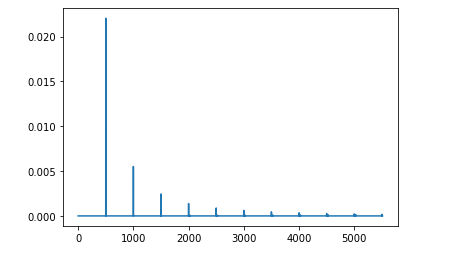
\includegraphics[width=\textwidth]{cos_spectrum_plot}
        \caption{Спектр косинусоидального сигнала}
        \label{fig:cos_spectrum_plot}
    \end{figure}

    Прослушаем данный сигнал.

    Выделим сегмент сигнала и выведем на экран.

    \begin{lstlisting}[language=Python, caption= Получение сигнала, label={lst:cos_segment_plot}]
        cos_wave.segment(duration=0.01).plot()
    \end{lstlisting}

    \begin{figure}[H]
        \centering
        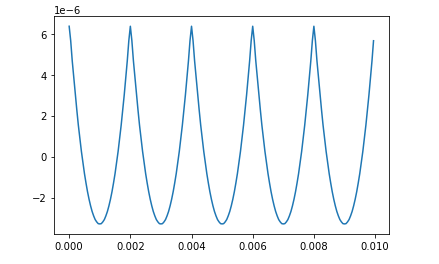
\includegraphics[width=\textwidth]{cos_segment}
        \caption{Сегмент косинусоидального сигнала}
        \label{fig:cos_segment}
    \end{figure}

    Полученный сигнал похож на параболы.
    Это верно лишь отчасти.
    Такого же результата можно добиться используя \texttt{ParabolicSignal} из \texttt{thinkdsp.py}.
    Создадим новый сигнал на основе \texttt{ParabolicSignal}.

    \begin{lstlisting}[language=Python, caption= Получение параболического сигнала используя ParabolicSignal, label={lst:par_signal_make}]
        from thinkdsp import ParabolicSignal

        par_wave = ParabolicSignal(freq=500).make_wave(duration=0.5, framerate=20000)
        par_wave.make_audio()
    \end{lstlisting}

    Послушаем сигнал и посмотрим на его график.

    \begin{figure}[H]
        \centering
        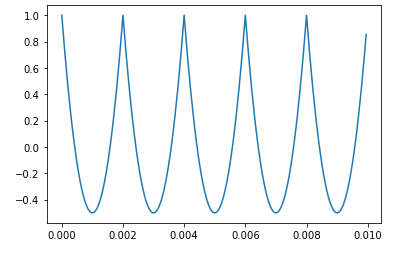
\includegraphics[width=\textwidth]{par_signal}
        \caption{Параболический сигнал}
        \label{fig:par_signal}
    \end{figure}

    Также посмотрим на его спектр.

    \begin{figure}[H]
        \centering
        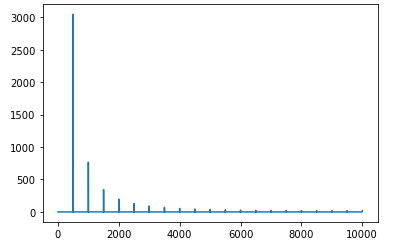
\includegraphics[width=\textwidth]{par_spectrum}
        \caption{Спектр параболического сигнала}
        \label{fig:par_spectrum}
    \end{figure}

    По результатам выполнения данного упражнения можно сделать вывод, что два последних полученных сигнала идентичны.

    Первый сигнал по звуку такой же как последние два, но график сигнала говорит об обратном.

    \section{Выводы}
    \label{sec:conclusions}
    В результате выполнения данной лабораторной работы мы изучили как надо работать с гармониками, как их обрабатывать, изменять параметры и т.д.
    Кроме того была реализован и проверен класс для получения пилообразного сигнала.
    Была создана функция для изменения спектра путем деления каждого элемента hs на соответствующую частоту fs.
    Был выведен параболический сигнал с помощью сложения косинусоидальных сигналов.

\end{document}